%%%%%%%%%%%%%%%%%%%%%%%%%%%%%%%%%%%%%%%%%
% Masters/Doctoral Thesis 
% LaTeX Template
% Version 2.5 (27/8/17)
%
% This template was downloaded from:
% http://www.LaTeXTemplates.com
%
% Version 2.x major modifications by:
% Vel (vel@latextemplates.com)
%
% This template is based on a template by:
% Steve Gunn (http://users.ecs.soton.ac.uk/srg/softwaretools/document/templates/)
% Sunil Patel (http://www.sunilpatel.co.uk/thesis-template/)
%
% Template license:
% CC BY-NC-SA 3.0 (http://creativecommons.org/licenses/by-nc-sa/3.0/)
%
%%%%%%%%%%%%%%%%%%%%%%%%%%%%%%%%%%%%%%%%%

%----------------------------------------------------------------------------------------
%	PACKAGES AND OTHER DOCUMENT CONFIGURATIONS
%----------------------------------------------------------------------------------------

\documentclass[
12pt, % The default document font size, options: 10pt, 11pt, 12pt
oneside, % Two side (alternating margins) for binding by default, uncomment to switch to one side (this also stops printing skips for duplex print)
english, % ngerman for German
singlespacing, % Single line spacing, alternatives: onehalfspacing or doublespacing
%draft, % Uncomment to enable draft mode (no pictures, no links, overfull hboxes indicated)
%nolistspacing, % If the document is onehalfspacing or doublespacing, uncomment this to set spacing in lists to single
%liststotoc, % Uncomment to add the list of figures/tables/etc to the table of contents
%toctotoc, % Uncomment to add the main table of contents to the table of contents
parskip, % Uncomment to add space between paragraphs
%nohyperref, % Uncomment to not load the hyperref package
headsepline, % Uncomment to get a line under the header
chapterinoneline, % Uncomment to place the chapter title next to the number on one line
%consistentlayout, % Uncomment to change the layout of the declaration, abstract and acknowledgements pages to match the default layout
]{MastersDoctoralThesis} % The class file specifying the document structure

\usepackage[utf8]{inputenc} % Required for inputting international characters
\usepackage[T1]{fontenc} % Output font encoding for international characters

\usepackage{mathpazo} % Use the Palatino font by default

\usepackage[backend=bibtex,style=authoryear,natbib=true]{biblatex} % Use the
                                % bibtex backend with the authoryear citation
                                % style (which resembles APA)


\usepackage{float} % Used to get image on title page to be on title page with [H]
\usepackage{glossaries} % Use the glossaries package for making a glossary

\addbibresource{example.bib} % The filename of the bibliography
\usepackage[autostyle=true]{csquotes} % Required to generate language-dependent quotes in the bibliography

\usepackage{hyperref} % Used to automatically add Figure, etc before references.

%----------------------------------------------------------------------------------------
%	MARGIN SETTINGS
%----------------------------------------------------------------------------------------

\geometry{
	paper=letterpaper, % Change to letterpaper for US letter
	inner=2.6cm, % Inner margin
	outer=3.8cm, % Outer margin
	bindingoffset=0cm, % Binding offset
	top=1.5cm, % Top margin
	bottom=1.5cm, % Bottom margin
	%showframe, % Uncomment to show how the type block is set on the page
}

%----------------------------------------------------------------------------------------
%	THESIS INFORMATION
%----------------------------------------------------------------------------------------

\thesistitle{Systems Engineering in\\Autonomous Underwater Vehicles} % Your thesis title, this is used in the title and abstract, print it elsewhere with \ttitle
\supervisor{Mr. Aman \textsc{Nijjar}} % Your supervisor's name, this is used in the title page, print it elsewhere with \supname
\examiner{} % Your examiner's name, this is not currently used anywhere in the template, print it elsewhere with \examname
\degree{Bachelor of Software Engineering} % Your degree name, this is used in the title page and abstract, print it elsewhere with \degreename
\author{Alec \textsc{Cox}} % Your name, this is used in the title page and abstract, print it elsewhere with \authorname
\addresses{} % Your address, this is not currently used anywhere in the template, print it elsewhere with \addressname

\subject{Control System Software Engineering} % Your subject area, this is not currently used anywhere in the template, print it elsewhere with \subjectname
\keywords{} % Keywords for your thesis, this is not currently used anywhere in the template, print it elsewhere with \keywordnames
\university{\href{http://www.uvic.ca}{University of Victoria}} % Your university's name and URL, this is used in the title page and abstract, print it elsewhere with \univname
\department{\href{https://www.uvic.ca/future-students/undergraduate/programs/pages/software-engineering.php}{Software
    Engineering - 4A}} % Your department's name and URL, this is used in the title page and abstract, print it elsewhere with \deptname
\group{\href{http://www.auvic.ca}{Autonomous Underwater Vehicle Interdisciplinary Club}} % Your research group's name and URL, this is used in the title page, print it elsewhere with \groupname
\faculty{Work Term - 1}} % Your faculty's name and URL, this is used in the title page and abstract, print it elsewhere with \facname

\AtBeginDocument{
\hypersetup{pdftitle=\ttitle} % Set the PDF's title to your title
\hypersetup{pdfauthor=\authorname} % Set the PDF's author to your name
\hypersetup{pdfkeywords=\keywordnames} % Set the PDF's keywords to your keywords
}

\makeglossaries
\newglossaryentry{AUV}{name={AUV},description={Acronym for autonomous underwater
  vehicle.}}
\newglossaryentry{DFA}{name={DFA},description={Acronym for deterministic finite
    state automaton. Simply described as a machine which which takes in an input
    sequence of symbols, for each of those symbols there is a defined
    transition, the complete parsing and transition through the DFA will either
    land the machine in a state that accepts the string, and otherwise rejects.
    See
    \href{https://en.wikipedia.org/wiki/Deterministic_finite_automaton}{Wikipedia}
    for a more detailed explanation}}

\newglossaryentry{IMU}{name={IMU},description={Acronym for inertial measurement
    unit. It is a sensor consisting of usually three of the following oriented
    orthogonal to the other sensor of the same type: accelerometers, gyroscopes, and sometimes
    magnetometers. It is used to measure pitch, roll, yaw, and magnetic field}}

\newglossaryentry{ROS}{name={ROS},description={Acronym for robot operating
    system. It is a C++ and python framework for development of robotics
    systems. It provides useful tools for device level abstraction,
    inter-process communication, and much more. See the libraries website for
    more information \href{https://www.ros.org}{here}}}

\newglossaryentry{opencv}{name={OpenCV},description={A computer vision library,
    name being shorthand for open source computer vision library}}

\newglossaryentry{JSON}{name={JSON},description={An acronym for JavaScript
    object notation. Despite its original creation for use with JavaScript it
    has become widely used by other programming languages. This is because of
    its format being easy to understand by humans, and easy to parse by
    computers.}}

\newglossaryentry{}{name={},description={}}


\begin{document}

\let\ref\autoref % wizardry for hyperref

\frontmatter % Use roman page numbering style (i, ii, iii, iv...) for the pre-content pages

\pagestyle{plain} % Default to the plain heading style until the thesis style is called for the body content

%----------------------------------------------------------------------------------------
%	TITLE PAGE
%----------------------------------------------------------------------------------------

\begin{titlepage}
\begin{center}

{\scshape\LARGE \univname\par}\vspace{0.5cm} % University name
\textsc{\Large Engineering & Computer Science Co-op\\Work Term Report\\Summer 2019}\\[0.5cm] % Thesis type

\HRule \\[0.4cm] % Horizontal line
{\huge \bfseries \ttitle\par}\vspace{0.4cm} % Thesis title
\HRule \\[1.5cm] % Horizontal line
 
\begin{minipage}[t]{0.4\textwidth}
\begin{flushleft} \large
\emph{Author:}\\
\href{http://www.hardsoftware.net}{\authorname}\\ % Author name
\textit{V00846488\\ENGR01\\\degreename}\\
\href{avlec@uvic.ca}{avlec@uvic.ca}
\end{flushleft}
\end{minipage}
\begin{minipage}[t]{0.4\textwidth}
\begin{flushright} \large
\emph{Supervisor:} \\
\href{http://www.auvic.ca}{\supname}\\ % Supervisor name - remove the \href bracket to remove the link  
\textit{}
\end{flushright}
\end{minipage}\\[2cm]
\groupname\\\deptname\\
\large \textit{Victoria, BC, Canada}\\[0.3cm] % University requirement text

{\large \today}\\[1cm] % Date

\begin{figure}[H]
  \centering
  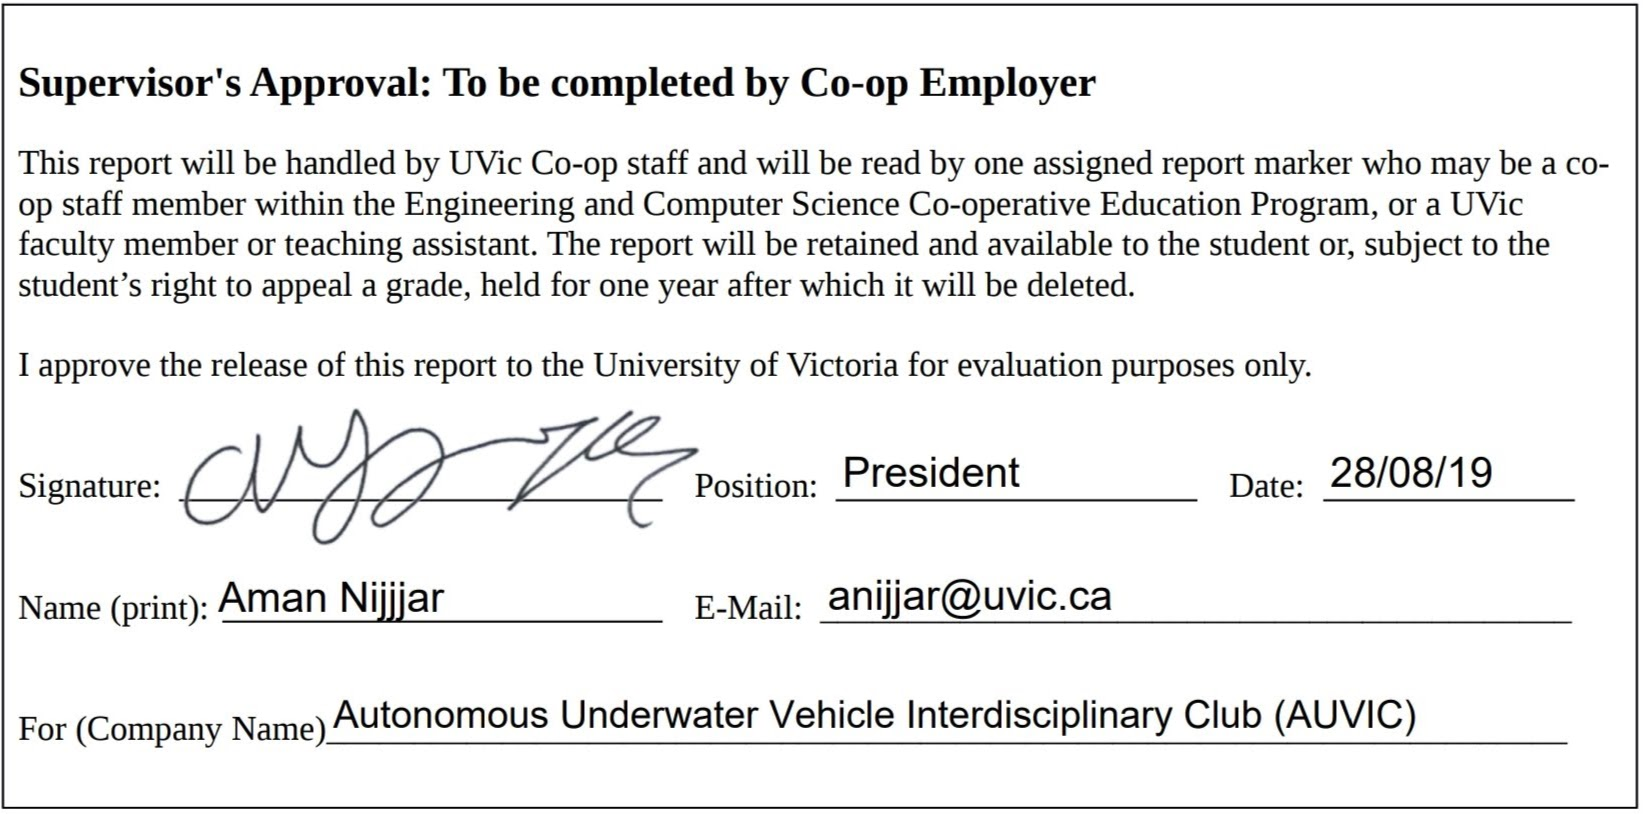
\includegraphics[width=100mm]{Figures/SupervisorApproval} % University/department logo - uncomment to place it
\end{figure}

\end{center}
\end{titlepage}

%----------------------------------------------------------------------------------------
%	ABSTRACT PAGE
%----------------------------------------------------------------------------------------

\begin{abstract}
\addchaptertocentry{Letter of Transmittal} % Add the abstract to the table of
% contents
Dear Imen Bourguiba,

Please accept the accompanying Work Term Report entitled ``Control Systems
Engineering in Autonomous Underwater Vehicles.''

The report is produced from work completed for AUVIC. AUVIC is located in the
University  of Victoria's Engineering Lab Wing. AUVIC is a club of undergraduate
students from different disciplines that work together to build and compete with
a AUV in the annual RoboSub competition in San Diego, California. The work done
on the software systems revolves around the control system and other systems
closely related to the control systems. This work involves creative problem
solving and generating innovative solutions to the complex challenge of
autonomous vehicle controls.

This report documents the reengineering process of AUVIC's control system.
This starts with providing the reader an understanding of the problem domain.
After the understanding has been established the report touches on the software
reengineering process. Following the reengineering process the conclusion
quickly covers over what was gained and learned from the whole process.
Finishing in the fifth section describing roadblocks encountered during the
process, and how they were overcome or how they could have been overcome.

I would like to acknowledge the work of other members of
AUVIC's software team those being: Rory Smith, Robert Keen, Adam Kwan, and Rob
Wassmann.

Sincerely,\\
\authorname
\end{abstract}

%----------------------------------------------------------------------------------------
%	LIST OF CONTENTS/FIGURES/TABLES PAGES
%----------------------------------------------------------------------------------------

\tableofcontents % Prints the main table of contents

\listoffigures % Prints the list of figures

\listoftables % Prints the list of tables

%\include{Chapters/Chapter0-Summary}


\newpage
\section*{Summary}

This report covers the re-engineering process of an existing software system,
one designed to provide autonomous control to an underwater vehicle.
Highlighting the success of the dynamic nature when it comes to on the fly
customization of the state machine.
Covering less positive results of the reengineering process; issues with
configuration and integrating the systems that were not
touched during the reengineering phase.
As well as lack of testing time, both out of and in the pool, led to rushed
last minute debugging at competition.
And also the good features from the old system that were unnoticed successes,
which resulted in problems during the competition.

Some of those good features that were missed during the re-engineering process
are as follows.

\begin{itemize}
\item Atomic movement instructions, which allowed for pre-programmed movements
  to be loaded dynamically from a \gls{JSON} file. Missing this in the final
  design led to states being significantly more complex because of their need to
  explicitly control how the AUV moved.
\item Simple interface to resources (e.g., detection results and AUV depth).
  This was possible since the control system provided an interface for them. It
  is worth noting the way this interface was implemented very poorly.
\item Simple interface to navigation commands (e.g., through atomic movement
  instructions). This allowed states to focus on getting the AUV setup to switch
  to the next state of execution. This was missed in the new design which lead
  to all movement related tasks to be done by hand.
\end{itemize}

The re-engineering process did however fix some of the problems with the
existing system. Those problems that were fixed are listed as follows.

\begin{itemize}
\item Static state control system was replaced with a control system with states
  that can be loaded at runtime.
  This is similar to how movement files were loaded from a JSON file, but these
  are loaded from a YAML configuration file.
\item Collection of too much responsibility within the control system.
  The solution was to separate the navigation components of the control system
  into different packages. However, this made access to system resources and
  navigation commands much more complex.
\end{itemize}

Summarizing, the positives from re-engineering the control system improved the
parts of the control system that they were engineered to fix.
However, the areas where the new control system were the parts left out from the
existing system.
The proper solution would need to bring the successes of both versions of the
control system into one unified system.

\printglossaries % Prints the glossary

%----------------------------------------------------------------------------------------
%	THESIS CONTENT - CHAPTERS
%----------------------------------------------------------------------------------------

\mainmatter % Begin numeric (1,2,3...) page numbering

\pagestyle{thesis} % Return the page headers back to the "thesis" style

% Include the chapters of the thesis as separate files from the Chapters folder
% Uncomment the lines as you write the chapters

% Chapter Template

\chapter{Introduction} % Main chapter title

\label{Chapter1} % Change X to a consecutive number; for referencing this chapter elsewhere, use \ref{ChapterX}

\section{Pretext}

AUVIC, is a team of students whose objective is to design, build, and compete an AUV. The team evolves as the students at the university join, enter Co-ops, and graduate. The team provides students with opportunity for hands on experience in submarine design, and work on complex autonomous systems.
Talk about team. Teams history. Role in team. Different sub-teams. Communication and meeting between sub-teams and members.

\section{Report Contents}

This report documents the migration from an old statically programmed control system with more responsibility than needed to a dynamic control system and two other systems taking over the excess responsibility. Starting off with explaining and understanding the problem domain from the perspective of the control system. The report then ventures into the domain of software reengineering where three different processes are described that occur. Those processes being: reverse engineering, restructuring, and forward engineering. The report then concludes with an analysis of the failures and successes of the produced system. All previous followed by the conclusion which expands on what was learned from the entire process.

\section{Glossary}

AUVIC - autonomous underwater vehicle interdisciplinary club\\
\gls{apple}


% Chapter Template

\chapter{Problem Domain} % Main chapter title

\label{Chapter2} % Change X to a consecutive number; for referencing this chapter elsewhere, use \ref{ChapterX}

%----------------------------------------------------------------------------------------
%	SECTION 1 - Operational Environment
%----------------------------------------------------------------------------------------

\section{Operational Environment}

The development for the AUV's high-level software system is developed in C++ and python. These languages are used as they work with our development environment. Our development consists of two primary libraries, ROS and OpenCV, running on Ubuntu 16.04. ROS, short for - Robot Operating System - is a amalgamation of different libraries useful for the development of robotic systems. We primarily use ROS for inter-process communication management, and hardware abstraction. OpenCV is a software package for the processing of images and video, used to give the AUV understanding from visual inputs.

The existing system consists of several different packages, two of which are impacted by the development of a new control system; those being "ai" (which would be renamed to controlsystem) and "nav" (which would be renamed to navigation). The ai package handled the state machine functionality of the AUV, also handling the detection systems as well.

Existing systems.
Inter-connectivity through ROS communication structures (that diagram).
Programming languages, and technologies.

Hardware.
Hydrophones, hydrophone boards, power board, IMU, Jetson TX2.
Diagram of hardware connections.

\chapter{Software Re-engineering}

\label{Chapter3}

This section covers a simplified process of software re-engineering.
Rhat is a process for taking an existing system developing an understanding of how it works, then refactoring that system and engineering changes, then implementing the system as to the conclusions made during refactoring.

Reverse engineering is the process of reviewing the existing software systems and documenting how they function. This can be done through diagramming, documenting, and refactoring. This process allows the engineer to understand the problem domain of the system more, and also provides information on parts of the software that need to be restructured and changed.

Restructuring is the process of taking an existing design and making changes to improve the design. This is the main transitional phase that will happen after the original understanding of how the current system works through reverse engineering. Restructuring will involve reorganizing code as granular or abstract as desired. Most restructuring will focus on making small changes to the system to make it more maintainable or run more efficiently. However, the restructuring of the current system will appear to be more of an overhaul.

% Need to expand this section.
Forward engineering is the process of taking the results of the system specification created from the two previous steps of the reengineering process integrating the system into the code-base.

\section{System Understanding}

The system is arranged for the most part into different functional groups, referred to as packages. There are some exceptions to this as seen in the "ai" package, where the responsibility of controls, vision, and movement is all amalgamated together.

The flow of information is handled quite elegantly within the system.
With lower level systems passing information up to and receiving back from
higher level systems. See \ref{fig:InformationFlow} for understanding the
general idea of how this flow happens.

\begin{figure}
\centering
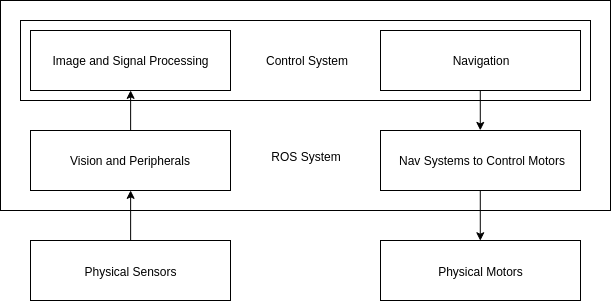
\includegraphics[width=100mm]{Figures/InformationFlow}
\decoRule
\caption[Original Information Flow]{Diagram showing how information flows in the reference frame of the control system.}
\label{fig:InformationFlow}
\end{figure}

The individual devices are handled via their own ROS nodes, which then make
the information from the devices available in a 'friendly' way.
This allows for specific driver-like programs to abstract the possibly
complex interface to the physical devices.


\section{Perceived Problems}

The control system featured no error catching or any kind of protocol to recover from an error state.
For most states the control system loops on a single state then after a condition is met will advance to the next state. This type of control system is autonomous controlling but it isn't designed for the kind of failures expected in the real world.

The control system works directly with the state information and directly handles both the condition to switch states and the assignment of the next state, see \ref{fig:DirectStateHandling}.

\begin{figure}
\centering
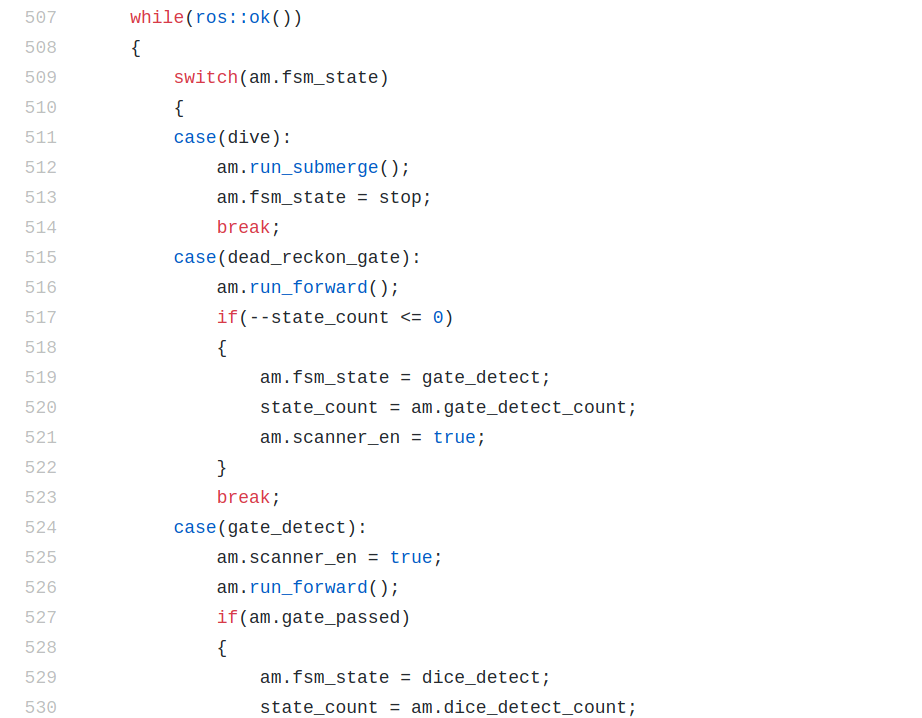
\includegraphics[width=150mm]{Figures/DirectStateHandling}
\decoRule
\caption[Direct State Handling]{Code segment showing the control systems way of handling states, controlling submarine functions, and getting information from other submarine systems.}
\label{fig:DirectStateHandling}
\end{figure}

The control system also directly handled the vision systems. The control system did offer a simple interface for the states in the state machine to utilize.


\section{Restructuring}

The control system has been assigned excessive responsibility; it performs the tasks of a control system, detection system, and navigation system. The detection systems within the control system shall be separated into a vision package and offer an interface through ROS inter process communication structures. Namely offer the same features the state machine was using, and expand the features on top of that. And the navigation system uses should also be pulled out, but an interface still be made available through ROS inter-process communication structures. To use the two new systems identified above they would need to be compatible with the existing system structure.

For the navigation system this required either using interface that existed and offered functionalities by replaced system, or a new system that acts as an interface to manage communication between old and new software systems. The latter involved much more consideration for best creating the system for usage in the future. While the former got the job done, and allowed to expand and slowly update functionality later on. Thus, the former of the two options was chosen, for the reasons given and because of time constraints for the project.

The detection systems' functionality and usage was restricted to within the control system. This allowed creation of a new system much simpler and allowed much freedom with the design of this system. Which is why the system used a simple interface to retrieve detection results, and change detection type. And this system was incorporated directly into the vision package, as having close proximity to the retrieved image files would mean for faster image processing.

The primary more generalized features to handle the support for different kinds of detection being: access to result of detection and the ability to change the current active detection algorithm which could also be set to none.

The updated version of the ROS communcation diagram was too large to embed into
this document, but it has been provided \href{https://drive.google.com/file/d/1_vJLSflxahA-7v2kYGV3wu5SfGcKEVf8/view?usp=sharing}{here}.

\begin{figure}
\centering
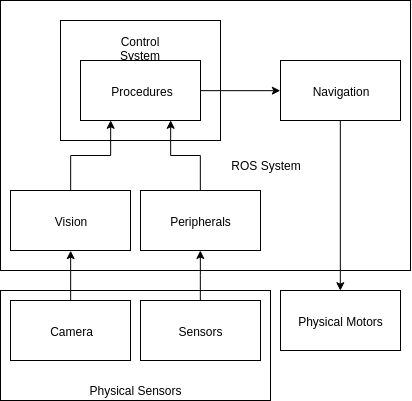
\includegraphics[width=100mm]{Figures/InformationFlowNew}
\decoRule
\caption[New Information Flow]{Diagram showing how information flows in the reference frame of the redesigned control system.}
\label{fig:InformationFlowNew}
\end{figure}

\begin{figure}
\centering
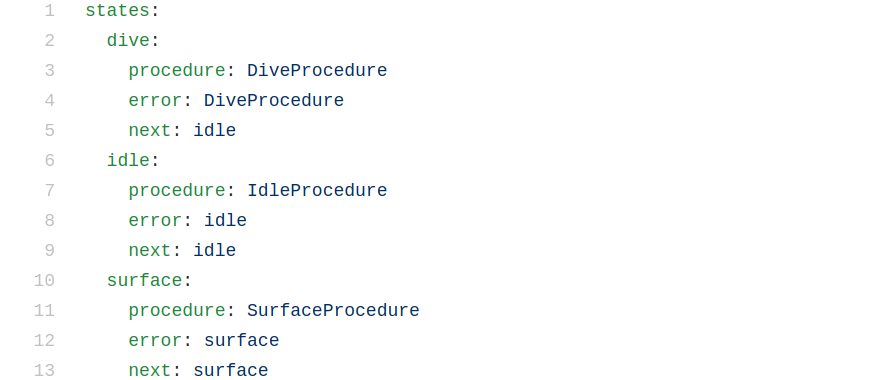
\includegraphics[width=150mm]{Figures/ExampleConfig}
\decoRule
\caption[Example Configuration File]{Shows a simple example idle configuration file. Demonstrating use of simple state organization and definition of state transitions.}
\label{fig:ExampleConfig}
\end{figure}

\section{Forward Engineering}


\chapter{Analysis}

\label{Chapter4}

This section covers both the failures and success stories of the system. It is worth noting that these were uncovered after the systems were integrated, and testing was being done preparing for the competition and at the competition.

\section{Failures}

\subsection{Resource Access}
The system design did not provide a simple mechanism for acquiring resources
from submarine.
Complex access lead to procedures being more complex than required, which caused
an increase in procedure development time.
This was because the complexity of the code caused implementation to take longer
because the procedures are compiled C++ code.
The issue can be mitigated by implementing an interface that provides access to
resources through a globally available singleton that abstracts access to all
available resources.
Alternatively, some abstraction offered by the control system to specific
resources which the procedure would need to request.

\subsection{Navigation}
The system design missed out on the easy interface for movement that was seen in
\ref{fig:DirectStateHandling}.
With the predefined movement commands it was easier to add new states with
different movement characteristics.
This was completely overlooked on the new system design, the idea of writing
procedures to complete individual tasks didn't inherently support this idea of
using predefined movement commands.
But seeing the results from a similar approach to navigation controls as was
seen in resource access.

This again caused more complex code which took longer to develop.
Although it offered the highest degree of control, it was unnecessary as most of
the procedures should have the movement abstracted away much like the detection
system.
This also led to procedures requiring to have access to ROS level inter-process
structures as seen in lines 168 to 170 of \ref{fig:NewProcedureOverhead}.

\subsection{Testing}
The system was designed and implemented correctly. The control, navigation, and
detection systems worked individually and ran without trouble. However, during
competition there were several problems getting the submarine launched with the
three new systems with the other existing systems.

Issues arose with the launch files that are used to start all systems required
for the AUV to function. Which was missed during testing of the systems
individually, and after implementing the changes mentioned above would need to
spend a significantly longer amount of time on.

Looking into getting testing frameworks for simulations like Gazebo would allow
us to ensure our systems are working with minimal amounts of in water testing.
Gazebo would allow us to run a model of the AUV in a simulated environment with
emulated sensors.
Which would allow testing to be done from each developers computer.
This is the highest priority item to ensure that issues are caught before
competition, to avoid from last minute rushed troubleshooting.

\begin{figure}
\centering
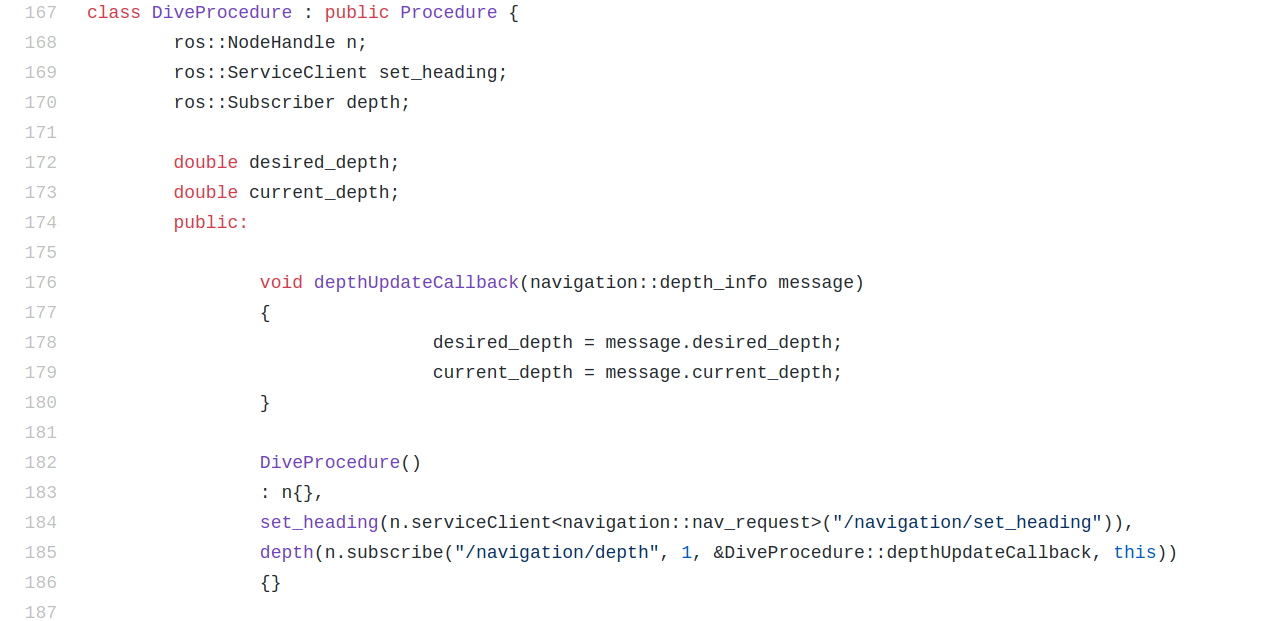
\includegraphics[width=150mm]{Figures/NewProcedureOverhead}
\decoRule
\caption[New Procedure Overhead]{Code segment shows new per-procedure overhead.}
\label{fig:NewProcedureOverhead}
\end{figure}

\section{Successes}

\subsection{Dynamic States}
The dynamic loading of the state machine accomplished its goal of making the
state machine operate in a less complicated way.
The loading of the states dynamically based off a configuration file allowed
functionality to be added and removed easily.
The only downside of this system is that despite the states being loaded in
dynamically the procedures needed to be statically typed and compiled to work
properly this way.
Changes that could make this better would be allowing the procedures to also be
loaded in dynamically through python or some other language.

\subsection{Procedures}

Procedures were a success in that the idea of what they should do was correct.
That is to say that despite the interfaces with accessing resources for and
navigation for moving the AUV the design was correct.

\subsection{Vision and Navigation Systems}

The separation of duty from the original control system into the vision and
navigation systems allowed for a more maintainable control system.
Though this did lead to issues as mentioned earlier about the complexity of
the systems interfaces.
If the procedures were to be provided with a simple interface to the navigation
system and vision system the procedures would be easier to write and more
effective.

\chapter{Conclusion}

\label{Chapter5}

The implementation of a new control system to handle the control of an AUV is no
simple task.
The design focused on fixing the failures of the existing system, while keeping
some of the successful features in the design.
However, the new design missed out on an abstracted interaction with the rest of
the submarine systems.
This lead to more complicated procedures, which hindered the on-the-fly
development of different procedures.

The dynamic loading of states also sparked the idea of creating a system for
writing dynamic procedures in some language that would be interpreted and loaded
into the control system on start up.
This would remove the requirement of changes of procedures resulting in
recompiling the control system package.
Would allow for procedures to be defined alongside the configuration files, and
allow rapid-fire prototyping with the ability to tune the procedures and
immediately test against a running system.

%----------------------------------------------------------------------------------------
%	THESIS CONTENT - APPENDICES
%----------------------------------------------------------------------------------------

\appendix % Cue to tell LaTeX that the following "chapters" are Appendices

% Include the appendices of the thesis as separate files from the Appendices folder
% Uncomment the lines as you write the Appendices

%% Appendix A

\chapter{Frequently Asked Questions} % Main appendix title

\label{AppendixA} % For referencing this appendix elsewhere, use \ref{AppendixA}

\section{How do I change the colors of links?}

The color of links can be changed to your liking using:

{\small\verb!\hypersetup{urlcolor=red}!}, or

{\small\verb!\hypersetup{citecolor=green}!}, or

{\small\verb!\hypersetup{allcolor=blue}!}.

\noindent If you want to completely hide the links, you can use:

{\small\verb!\hypersetup{allcolors=.}!}, or even better: 

{\small\verb!\hypersetup{hidelinks}!}.

\noindent If you want to have obvious links in the PDF but not the printed text, use:

{\small\verb!\hypersetup{colorlinks=false}!}.

%\include{Appendices/AppendixB}
%\include{Appendices/AppendixC}

%----------------------------------------------------------------------------------------
%	BIBLIOGRAPHY
%----------------------------------------------------------------------------------------

%\printbibliography[heading=bibintoc]

%----------------------------------------------------------------------------------------

\end{document}  
